\textbf{Beispiel 2}\\ \\
a)\\ \\
Die beiden gesuchten Parameter lauten hier
\[
	R_U = \frac{1}{A_s\alpha_S} \quad,\quad C_s = m_Sc_S
\]
b) \\ \\
Zuerst wird die Sichtfaktormatrix benötigt. Da der Glühfaden nicht auf sich selbst strahlt lautet der entsprechende Sichtfaktor
\[
	F_{GG} = 0
\]
Somit lauten die restlichen Sichtfaktoren die durch die Summationsregel und dem Reziprozitätsgesetz bestimmt werden
\begin{align*}
	F_{G\infty} &= 1 \\
	F_{\infty G} &= 0 \\
	F_{\infty\infty} &= 1
\end{align*}
Somit gilt für die Sichtfaktormatrix
\[
	\textbf{F} = \begin{bmatrix}
		0 & 1 \\
		0 & 1
	\end{bmatrix}
\]
\newpage
\noindent
c) \\ \\
Der thermische Widerstand des Leiters wird analog zum spezifischen elektrischen Widerstand bestimmt. Damit erhaltet man für den thermischen Widerstand
\[
	R_L = \frac{L}{\lambda A_L}
\]
d) \\ \\
Wärmeübergänge werden als Widerstände, Bereiche mit veränderlicher Temperatur als Kapazitäten, konstante Temperaturen als Spannungsquellen und zugeführte Leistungen als Stromquellen dargestellt. Daher ergibt sich für die RC-Ersatzschaltung dieses Problems
\begin{figure}[h]
	\centering
	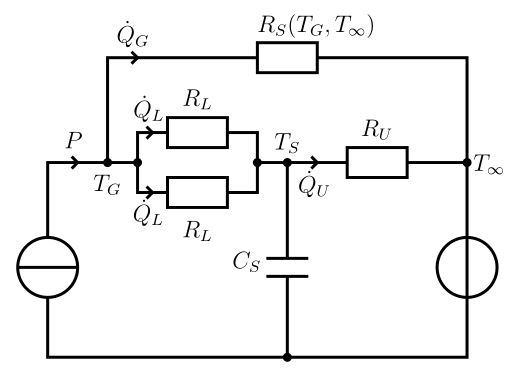
\includegraphics[width=10cm]{tikz/07_02_2020_2d}
\end{figure}
\newline
e) \\ \\
Die Differentialgleichung wird aus den Maschen und Knoten, analog wie im elektrischen Fall, aus der Schaltung hergeleitet. Diese lautet hier
\[
	\dot{T}_S(t) = \frac{1}{C_S}\left(\frac{T_G(t) - T_S(t)}{\frac{R_L}{2}} - \frac{T_S(t) - T_\infty}{R_U}\right)
\]
f)\\ \\
Aus der Ersatzschaltung ergibt sich für die gesuchte Gleichung
\[
	P - \frac{T_G - T\infty}{R_U + \frac{R_L}{2}} - \frac{T_G - T_\infty}{R_S(T_G,T_\infty)}
\]